\documentclass[dvipdfmx, a4,12pt]{jarticle}
\usepackage{amsmath,amssymb}
\usepackage{amsthm}

\usepackage{tikz}

\begin{document}

%%-----
\begin{figure}[h]
	\centering  	%中央ぞろえ
	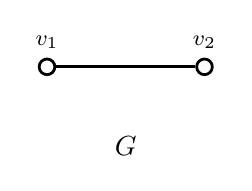
\begin{tikzpicture}[line width=1pt, node distance=15mm, label distance=0.1pt]

		%点
		\footnotesize	% 文字の大きさを小さく
		\coordinate (v0) at (0, 0); %原点にv0と名前をつける
		\tikzset { 
			styleVertexs/.style= {
				draw, circle, inner sep=2pt
			}		%点の形を丸、大きさを2pt
		};
		%ループで点を書く
		\foreach 
			\vertexName/\startVertexName/\angle/\radius in { 
				1/0/0/0, 2/1/0/20 } {
			%各点の上に名前を書く
			\tikzset{ stylev\vertexName/.style={ 
				label= { 
					[name=labelv\vertexName] %ラベル位置に名前をつける
					above : $v_{\vertexName}$ 
				}
			} };

			%\startVertexNameから極座標で点を置く
			\path (v\startVertexName) -- ++(\angle : \radius mm)
				node [
					styleVertexs, stylev\vertexName
				] (v\vertexName) {};	%点の位置に名前をつける
		}

		%ループで辺を書く
		\foreach \startVertexName/\endVertexName in 
			{1/2} {
			%\draw (v\startVertexName) -- (v\endVertexName);	%線を引くだけ
			%線の中央に名前をつけたいとき(下のグラフの名前をつけるときに使う)
			\draw (v\startVertexName) 
								-- coordinate(v\startVertexName v\endVertexName) 
						  (v\endVertexName);
		}

		%グラフの名前
		\path (v1v2) -- ++(-90 : 10mm)	%v1v2は辺v1v2の中央
			node(G) { {\normalsize $G$} } ;

	\end{tikzpicture}
	\caption{ ここに図の名前を記入. }
	\label{ラベルを指定}
\end{figure}
%%-----
%
\end{document}